\documentclass{article}
\usepackage[utf8]{inputenc}
\usepackage{url}
\usepackage{graphicx}
\usepackage{hyperref}
\usepackage{amsmath}
\graphicspath{ {./} }


\title{Automatisation du prétraitement de photographies de portraits de mandrills}
\author{Maxime Boucher}
\date{Compte rendu 9}

\begin{document}

\maketitle

Depuis la dernière fois j'ai travaillé sur :
\begin{itemize}
\item la mise en place de docker pour permettre que le code fonctionne partout (tout OS, n'importe quand). \\

Exemple de build par docker
\begin{center}
    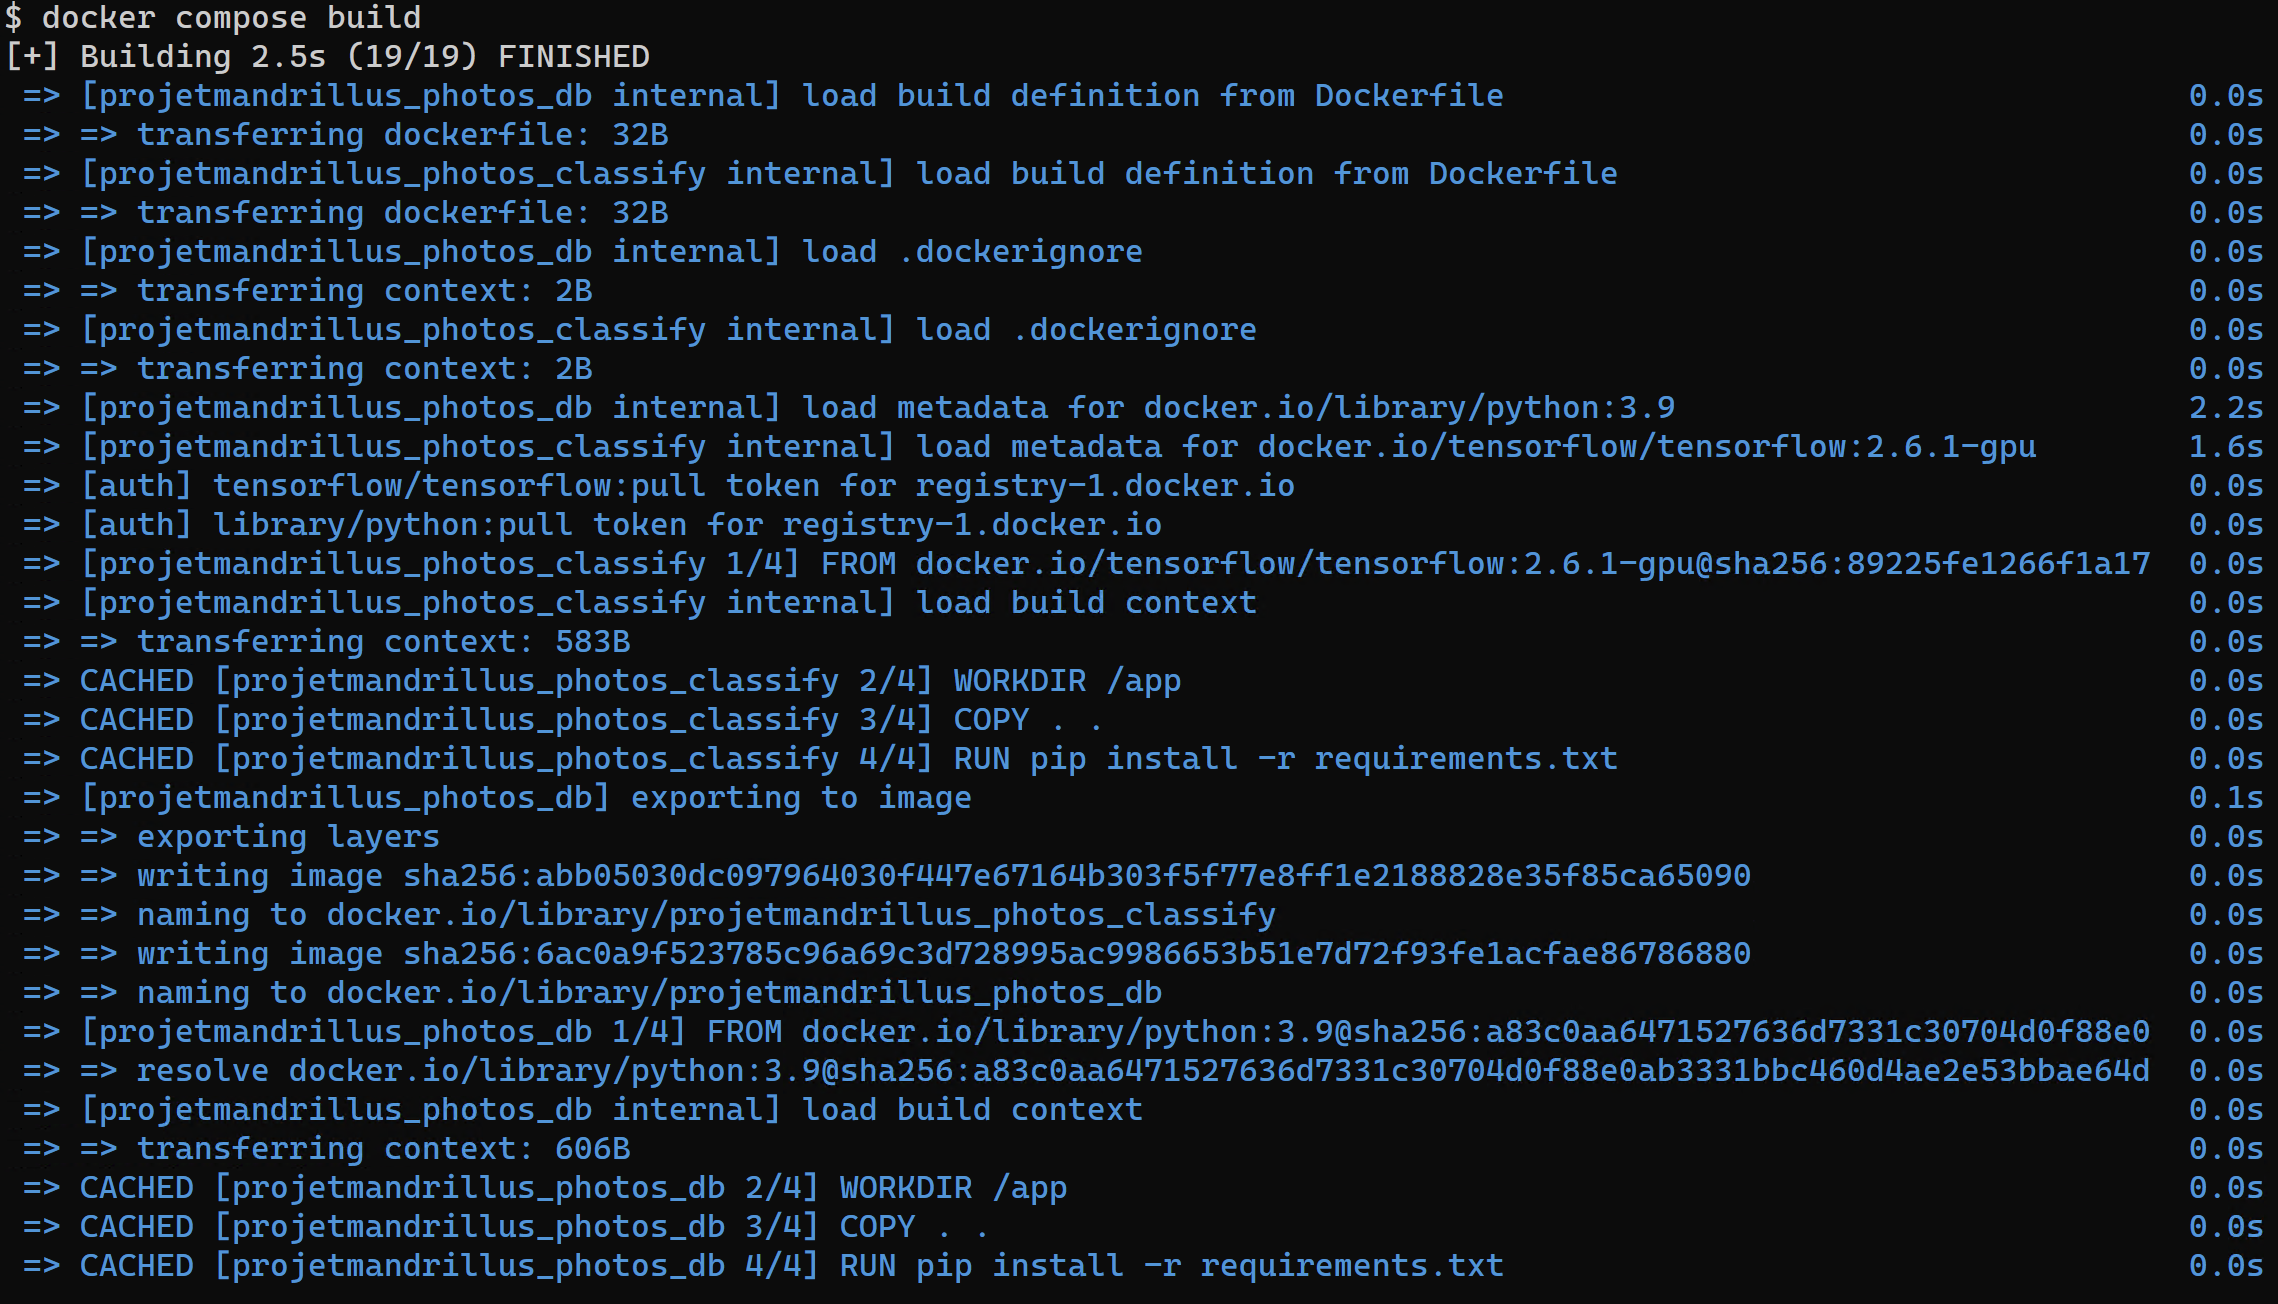
\includegraphics[width=345]{imgs/qualité/cr9/build.png}
\end{center}

Exemple de Dockerfile
\begin{center}
    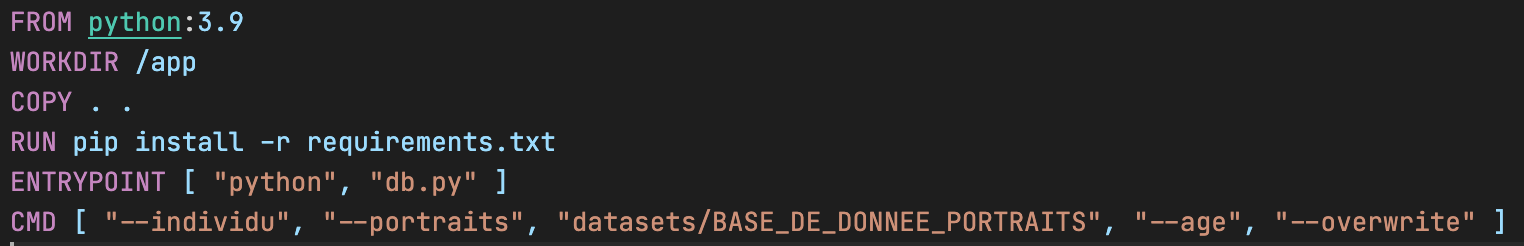
\includegraphics[width=345]{imgs/qualité/cr9/dockerfile.png}
\end{center}

Exemple de docker-compose.yml
\begin{center}
    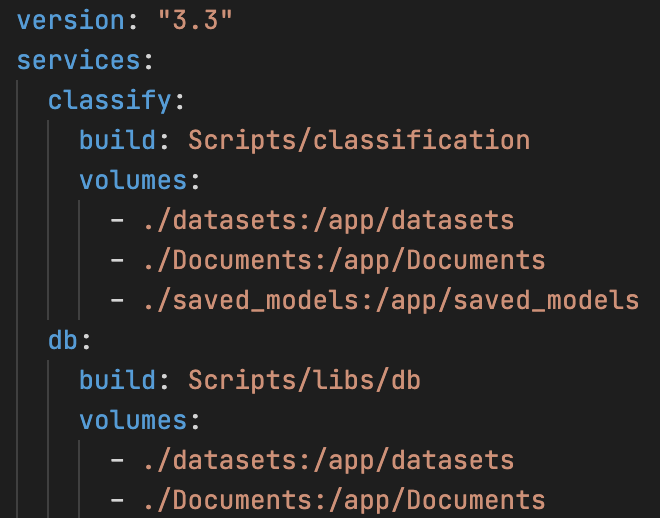
\includegraphics[width=345]{imgs/qualité/cr9/compose.png}
\end{center}

\item le changement de la manière dont on représente les keywords : "1FaceQual" devient par exemple "FaceQual:". Et ce, sur la base de données originales. Les mots clés sont ensuite indiqués tel que : 1FaceQual1 deviendrait FaceQual:1

\item le changement des noms de fichiers de sorte que ça respecte la charte que l'on a adapté au 28/04 \\
Charte pour nommer les fichiers
\begin{center}
    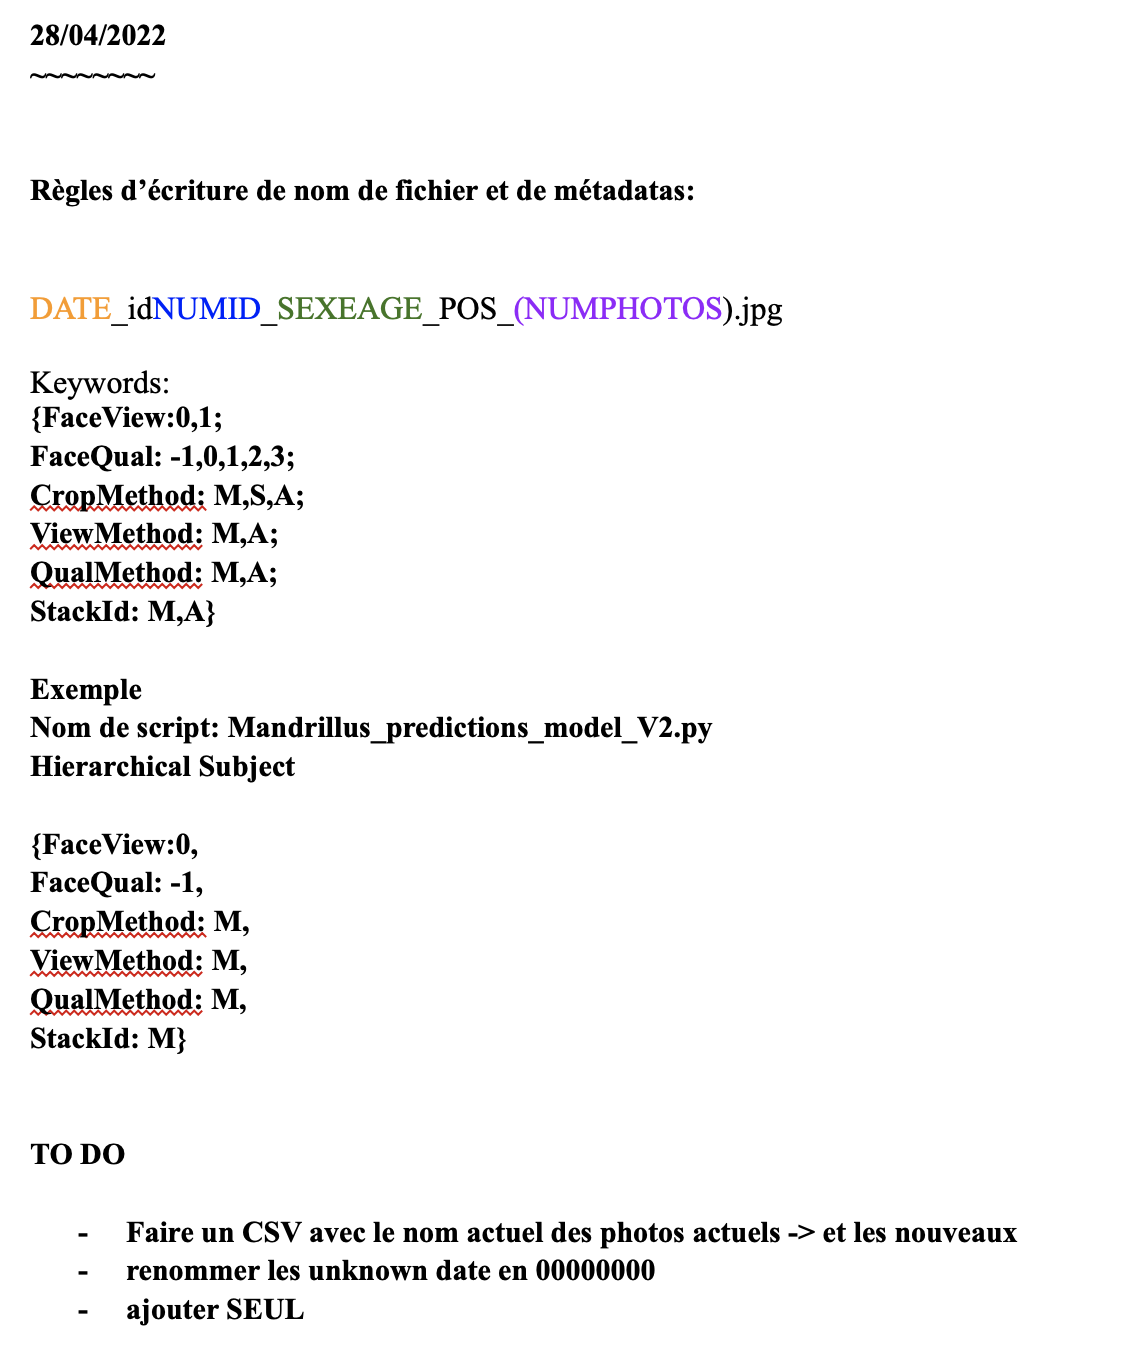
\includegraphics[width=345]{imgs/qualité/cr9/charte.png}
\end{center}
\end{itemize}

\end{document}
